\documentclass[conference]{IEEEtran}
\usepackage{cite}
\usepackage{amsmath,amssymb,amsfonts}
\usepackage{algorithmic}
\usepackage{booktabs, bm}
\usepackage{caption}
\usepackage{graphicx}
\usepackage{listings}
\usepackage{textcomp}
\usepackage{xcolor}
\usepackage[utf8]{inputenc}

\definecolor{codegreen}{rgb}{0.7,0.7,0.7}
\definecolor{codegray}{rgb}{0.5,0.5,0.5}
\definecolor{codepurple}{rgb}{0.58,0,0.82}
\definecolor{backcolour}{rgb}{0.985,0.985,0.985}
 
\lstdefinestyle{mystyle}{
    backgroundcolor=\color{backcolour},   
    commentstyle=\color{codegreen},
    keywordstyle=\color{magenta},
    numberstyle=\tiny\color{codegray},
    stringstyle=\color{codepurple},
    basicstyle=\ttfamily\footnotesize,
    breakatwhitespace=false,         
    breaklines=true,                 
    captionpos=b,                    
    keepspaces=true,                 
    numbers=left,                    
    numbersep=5pt,                  
    showspaces=false,                
    showstringspaces=false,
    showtabs=false,                  
    tabsize=2
}
 
\lstset{style=mystyle}
\def\BibTeX{{\rm B\kern-.05em{\sc i\kern-.025em b}\kern-.08em
    T\kern-.1667em\lower.7ex\hbox{E}\kern-.125emX}}
\begin{document}

\title{CENG435 Term Project Part 1\\}

\author{\IEEEauthorblockN{Necla Nur Akalın}
2171148
}
\maketitle

\section{Introduction}
In part 1 of the Ceng435 term project, firstly it was expected to find the links costs between five nodes. By using user datagram protocol(UDP), with the given topology and IP addresses, I was supposed to send the messages from one node to another to find link costs. Secondly, I was expected to find the shortest path from the node $s$ to node $d$, and do given experiments to on that shortest path. Finally, it was asked us to plot the  relation of network emulation delay and the end-to-end delay with a 95\% confidence interval for each of the different communications given.

\section{Network Topology and Link Cost Scenario}
The network topology consists of five nodes, which are already prepared and given to us as an $.xml$ file.
\begin{figure}[h!]
  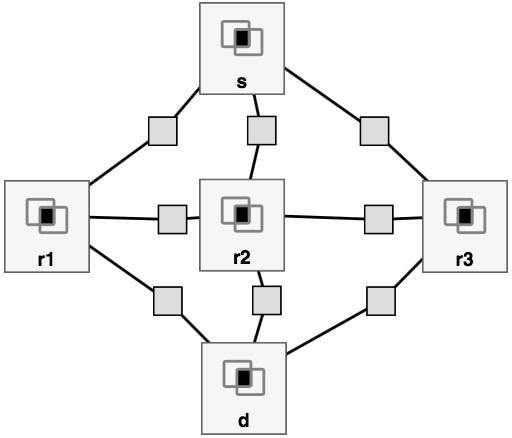
\includegraphics[width=0.6\linewidth]{topology.png}
  \centering
  \caption{The Network Topology}
  \label{fig:Topology}
\end{figure}

In order to create the topology on Geni Platform, I copied the content of the $.xml$ file and pasted it to text box under the add resources section of Geni Platform. After the reserving process of the topology, in order to give the initial conditions to nodes $r1$ and $r2$, I ran the $configure1.sh$ and $configure2.sh$ scripts by connecting the nodes by ssh, which are given to us with the homework.

My first aim was to find the shortest path between the node $s$ and the node $d$. In total, I needed to measure the costs of $8$ different links, and so I had a lot of different scenarios that I can apply. I decided to use $r1$ and $r3$ only as clients, $s$ and $d$ only as servers and $r2$ both as a client and a server. In other words, for both $r1$ and $r3$, I sent messages to $s$, $r2$ and $r3$ and saved the costs in the nodes $r1$ and $r3$; for $r2$, I both received messages from $r1$ and $r3$, and I sent messages to $s$ and $d$ and saved the link costs in $r2$, and finally for both $s$ and $d$ I only received messages from the nodes $r1$, $r2$ and $s$.

\section{Measuring Link Costs}
To measure the link costs between nodes, it was asked us to develop a UDP socket application. 

User Datagram Protocol is used to establish low-latency and loss-tolerating connections between internet applications. Different than Transmission Control Protocol(TCP), UDP does not wait for server to confirm that the message from the client is really sent. Thus, I can say that UDP is less trustworthy and as it does not contain an error-checking algorithm, it is faster when compared with TCP. In addition, in case of a loss, there is no recovery in UDP as it directly sends message to recipient.

In socket programming, two nodes are connected to each other by given IP addresses and ports so that they can build a network and communicate with each other. A socket in socket programming is called to the end-point node of the connection, in this case, I had server sockets and client sockets. Server sockets are listening for an incoming message on a specific port with an IP while client sockets are sending the messages to server sockets.

\subsection{Programming Language}
I decided to use Python as the programming language to implement the codes as there's the library called $socket$ which allows us to send and receive messages between nodes easily. In the scripts, I created sockets for every server node with the code below:
\begin{lstlisting}[language=Python, caption=Creating sockets in Python]
import socket
# Creating sockets for servers
s_socket = socket.socket(family = socket.AF_INET, type = socket.SOCK_DGRAM)
d_socket = socket.socket(family = socket.AF_INET, type = socket.SOCK_DGRAM)
r2_socket = socket.socket(family = socket.AF_INET, type = socket.SOCK_DGRAM)
\end{lstlisting}

To measure the link costs, I wrote 5 different python scripts for each of the nodes. These scripts should be ran inside the nodes by first running the servers and then the clients, in other words, first the scripts for $s$ and $d$ should be ran, then $r2$ and then the scripts for $r1$ and $r3$ should be ran.

\subsection{Multi Threading}
Multi threading is a programming model that divides the processor to execute different tasks at the same time. To handle different request at the same time, I need to create seperate threads. A thread is a group of instructions that can be executed independently from the main code. In order to send/receive messages from different nodes, also to use a node both as a client and a server at the same time, I need to use multi threading in the scripts, and so I need to create multiple threads. Python has a library called $threading$ and I used this library in the scripts.

For the nodes $r1$ and $r3$, I started three threads. As we're doing the same tasks(sending messages to servers) with the only difference of IP addresses, ports and sockets for all of the threads, I wrote only one function and sent IP addresses, ports and sockets as inputs with the threads. You can see the threading codes and how I did call the $server$ function below:
\begin{lstlisting}[language=Python, caption=Multithreading in Python]
import threading
# IP addresses and ports of servers
s_addressPort = ("10.10.1.1", 20001)
d_addressPort = ("10.10.4.2", 20011)
r2_addressPort = ("10.10.8.2", 20021)
    ...
# Function to send and receive messages from servers
def server(addressPort, socket, id):
    ...
# Creating threads
thread_s = threading.Thread(target = server, args = (s_addressPort, s_socket, 's'))
thread_d = threading.Thread(target = server, args = (d_addressPort, d_socket, 'd'))
thread_r2 = threading.Thread(target = server, args = (r2_addressPort, r2_socket, 'r2'))
# Starting threads
thread_s.start()
thread_d.start()
thread_r2.start()
\end{lstlisting}

\subsection{Round Trip Time Value}
In order to measure the link costs I had to find round trip times(RTTs) of messages sent from clients to servers. In short, RTT is the length of time that a message takes to be sent and to be received back. In the codes to measure RTT, I used the library $time$. I measured the time right after I send a message and also right after I received a reply message. Since I measured the time as a floating point number expressed in seconds since the epoch, I subtract the first value from the second one to find the RTT. You can see the details of this code below:
\begin{lstlisting}[language=Python, caption=Finding RTT in Python]
import time
...
bufferSize = 1024
s_cost = [] # Array to keep link costs
t_num = 1000 # Number of messages to send
def server(addressPort, socket, id):
    ...
    count = 0
	while count < t_num:
	# Send to server using created UDP socket
		socket.sendto(bytesToSend, addressPort)
		start = time.time()
		msgFromServer = socket.recvfrom(bufferSize)
		end = time.time()
		if id == 's':
			s_cost.append(float((end-start))/2)
\end{lstlisting}

While appending RTT values to the cost storage arrays, I divided them into two so that I could find one-way delay of the links, i.e. link costs. I also wrote all of those links costs of every message sent, and their total and average costs in the files names $x\_to\_y\_costs.txt$ where $x$ and $y$ stands for node names.

\subsection{Node R2 Exception}
As I mentioned before, I used both $r1$ and $r3$ as client nodes and both $s$ and $d$ as server nodes. However, I had to use $r2$ both as a client and a server. In other words, while I was only sending and waiting for a response message in $r1$ and $r3$ and while I was only receiving and sending response messages in $s$ and $d$, I was doing both on the node $r2$. Thus, in the script for $r2$, I wrote two different functions named $being\_s$ and $being\_c$ which are stands for functions acting like a server and client in order. Once again, I had to use multi threading for those two functions, so that $r2$ could get messages from clients and send messages to servers at the same time. Thus, different than other nodes, I also used multi threading for $r2$ to act both like a client and a server at the same time.

\section{Finding Shortest Path}
By sending 1000 messages from clients to servers, I achieved the average costs in seconds that can be seen in the graph below.

\begin{figure}[h!]
  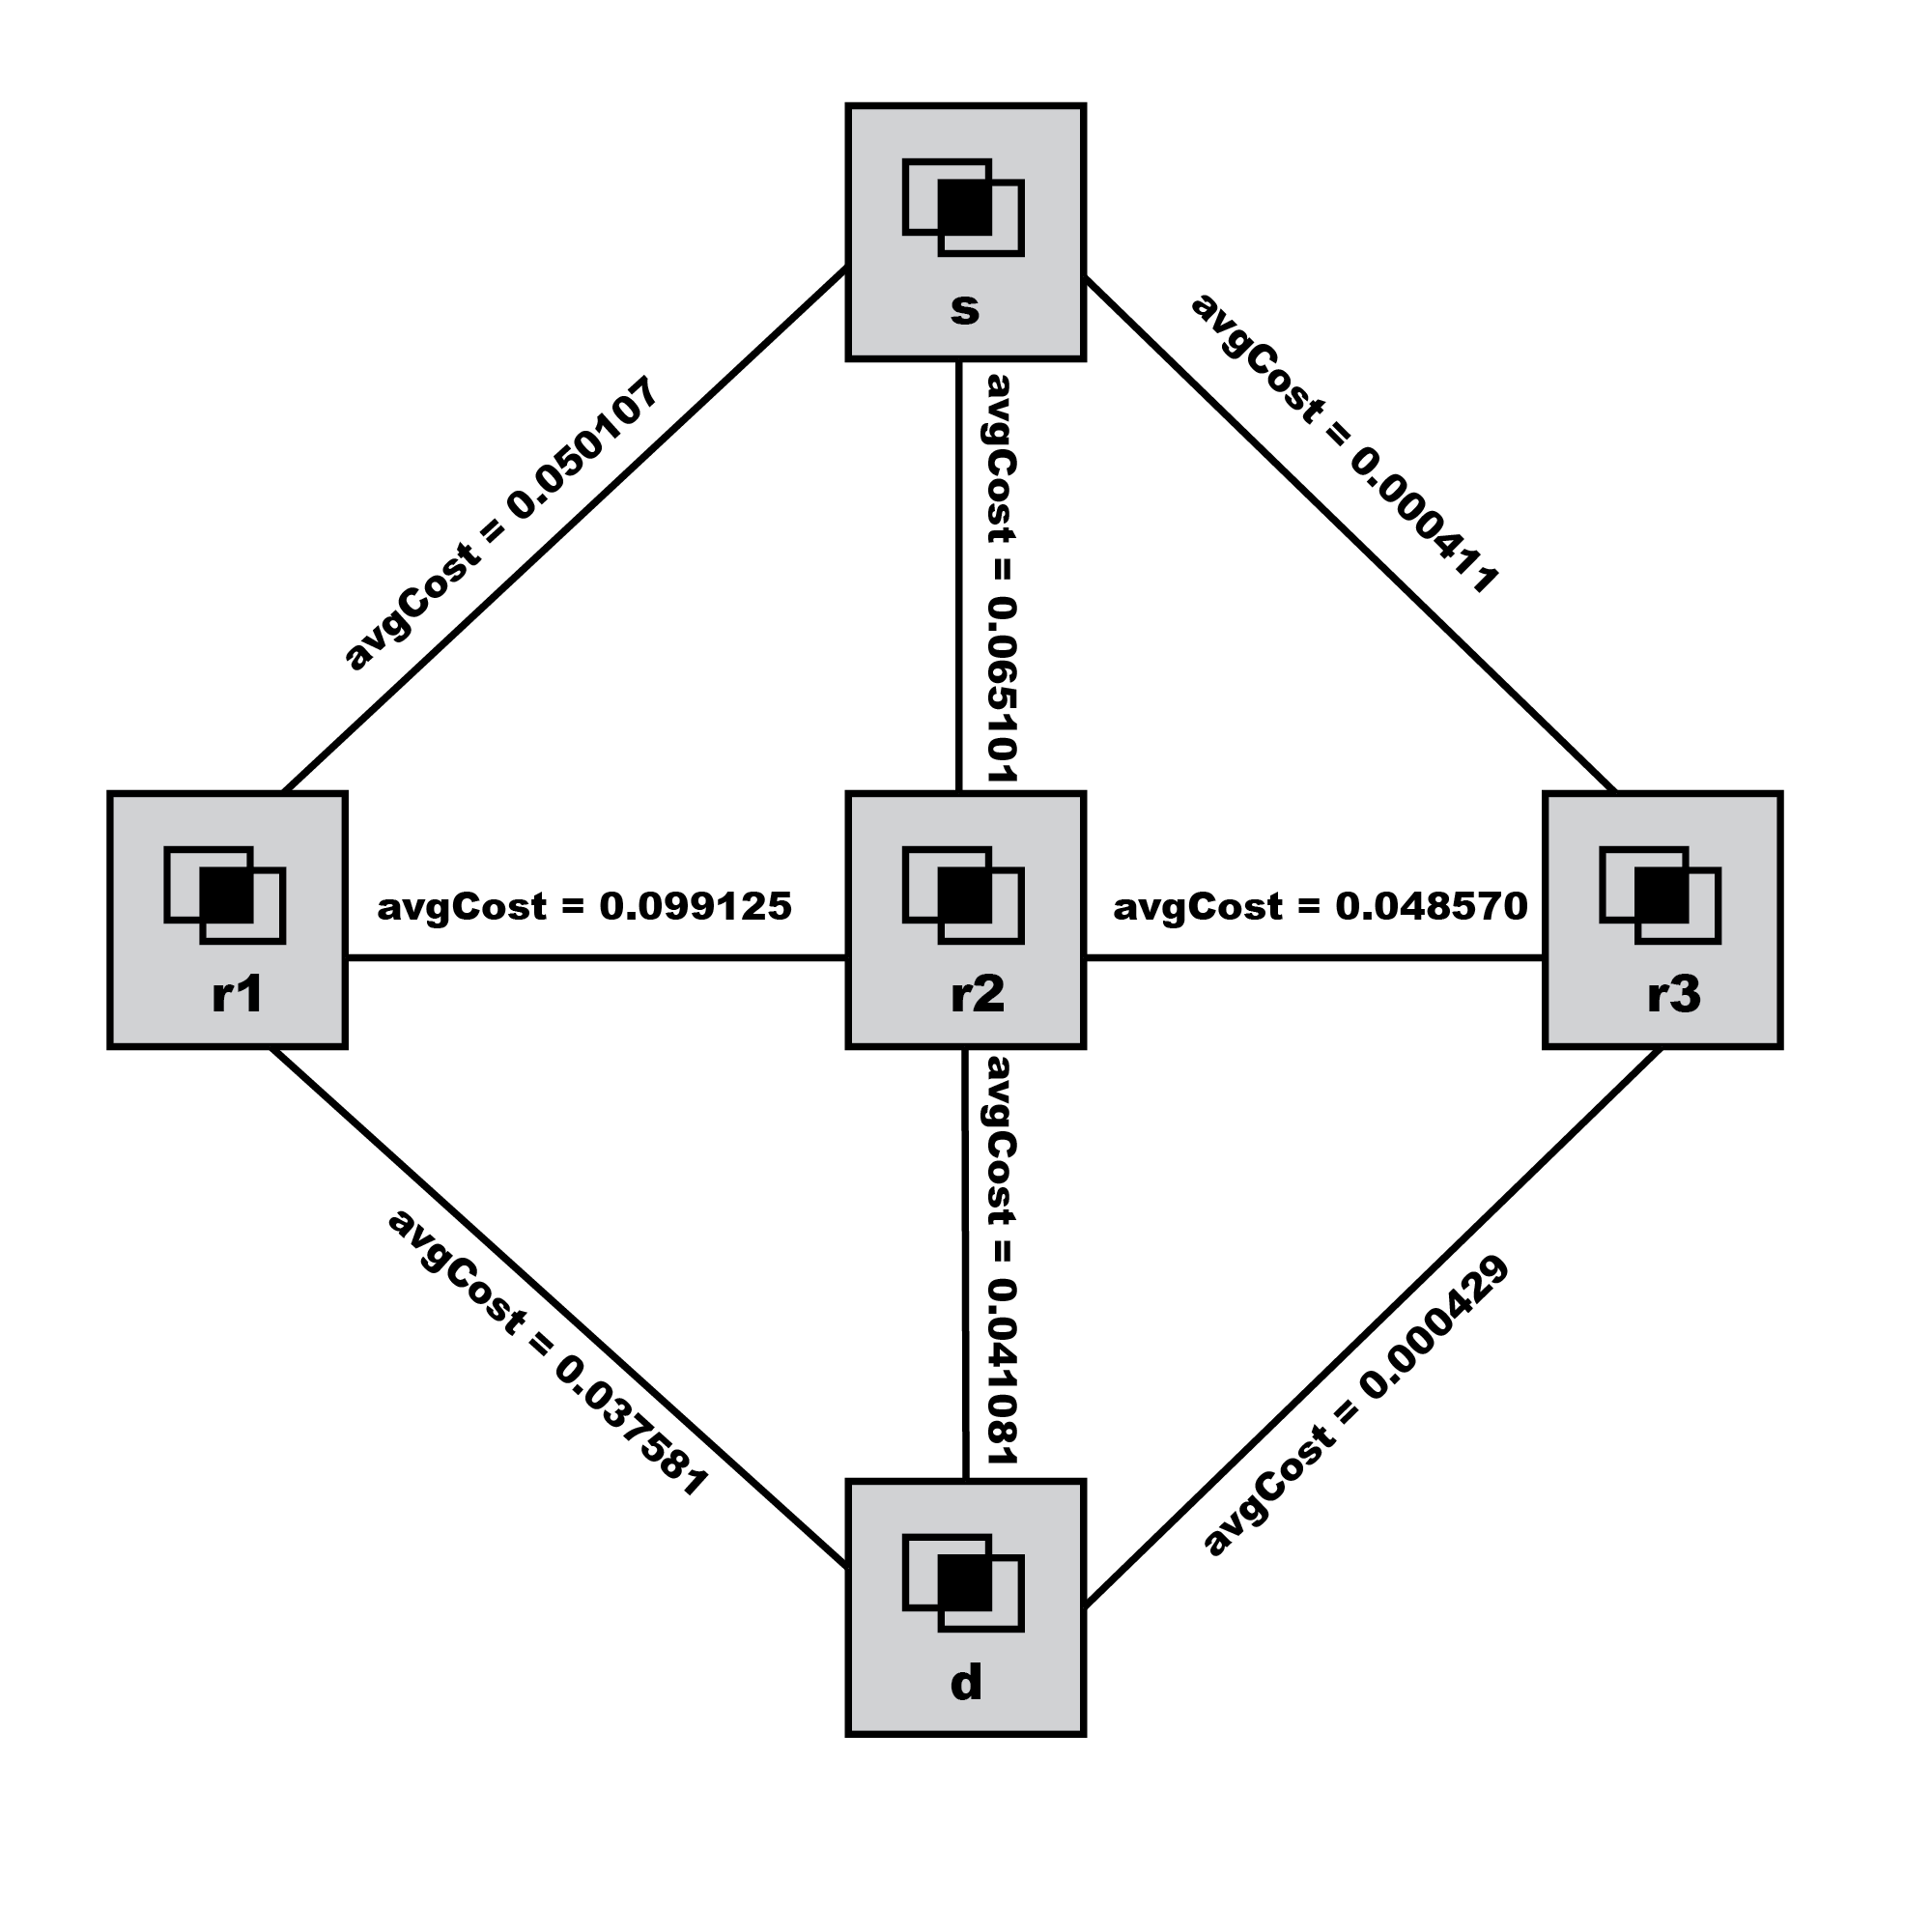
\includegraphics[width=\linewidth]{shortestPath-01.png}
  \centering
  \caption{Line Costs}
  \label{fig:Topology}
\end{figure}

In milliseconds, these are the costs I got after 1000 messages: \\ r1-s $\approx$ 50ms\\ r1-r2 $\approx$ 99ms\\ r1-d $\approx$ 38ms\\ r3-s $\approx$ 0.4ms\\ r3-r2 $\approx$ 49ms\\ r3-d $\approx$ 0.43ms\\ r2-s $\approx$ 65ms\\ r2-d $\approx$ 41ms.

\subsection{Dijkstra Algorithm}
It was asked us to find the shortest path by using Dijkstra algorithm. In Dijkstra algorithm, I build a shortest path tree from source to destination, in this case, from node $s$ to node $d$. I create two groups, in which I keep the shortest path's route in one of them, and keep the vertices which are not included in shortest path tree yet in the other one.

I can write Dijkstra's algorithm to find the shortest path in the form of a table as follows.
\begin{table}[h!]
\begin{tabular}{ll|llll}
v & & r1 & r2 & r3 & d \\ \hline
\multicolumn{1}{l|}{1} & s & $50_s$ & $65_s$ & \bm{$0.4_s$} & $\infty_s$ \\
\multicolumn{1}{l|}{2} & r3 & $50_s$ & $65_s$ & \bm{$0.4_s$} & \bm{$0.83_{r3}$} \\
\multicolumn{1}{l|}{3} & d  & \bm{$50_s$} & $65_s$ & \bm{$0.4_s$} & \bm{$0.83_{r3}$} \\
\multicolumn{1}{l|}{4} & r1 & \bm{$50_s$} & \bm{$65_s$} & \bm{$0.4_s$} & \bm{$0.83_{r3}$} \\
\multicolumn{1}{l|}{5} & r2 & \bm{$50_s$} & \bm{$65_s$} & \bm{$0.4_s$} & \bm{$0.83_{r3}$} 
\end{tabular}
\centering
\caption{Dijkstra's Algorithm}
\label{fig:Topology}
\end{table}

By using this algorithm, I see that the shortest path I get from the node $s$ to $d$ is only via the node $r3$ with the total cost of $0.83ms$.

\section{Experiments}
In these experiments, I was expected to plot a figure that provides the relation of network emulation delay and the end-to-end delay with a 95\% confidence interval for each of the different communications.

A network emulation is the act of introducing a device to networks to create a delay by altering packet flow. The main usage of these emulators is to observe different network latency levels so that one can test his/her application in a more realist environment. On the other hand, as I described before an end-to-end delay is the delay that a message takes to be sent and recieved back.

In order to create emulation delays, I used tc/netem commands. You can see the tc command I used for experiment 1 below:
\begin{lstlisting}[language=c, caption=Emulation Delay Command]
# tc qdisc add dev eth1 root netem delay 20ms 5ms distribution normal
\end{lstlisting}

In this term project, I experimented three different emulation delays. Thus, I used different tc commands for each of the experiments by only changing the delay amounts.

In experiment 1, I used an emulation delay of $20ms+-5ms$. After sending multiple messages, between the nodes $s$ and $r3$, I got an average cost of $0.3437ms$ and between the nodes $r3$ and $d$, I got $0.3831ms$ delay. Thus, in total, between $s$ and $d$ I had $0.7268ms$ of end-to-end delay.

In experiment 2, I used an emulation delay of $40ms+-5ms$. Between the nodes $s$ and $r3$, I got an average cost of $0.3880ms$ and between the nodes $r3$ and $d$, I got $0.3955ms$ delay. Thus, in total, between $s$ and $d$ I had $0.7835ms$ of end-to-end delay. When compared with the first experiment, achieving a higher end-to-end delay was expected. Even though, the result I got after the second experiment is bigger than the first experiment's result, it is still not high enough as it was expected.

In experiment 3, on the other hand, I used an emulation delay of $50ms+-5ms$. Between $s$ and $r3$ nodes, an $0.3787ms$ of end-to-end is achieved. Between the nodes $r3$ and $d$, the end-to-end delay became $0.3828ms$. In total, the end-to-end delay between $s$ and $d$ for experiment 3 became $0.7615ms$. I was expecting to get an higher end-to-end delay in experiment 3 than I achieved both in experiment 1 and experiment 2. Even though, experiment 3's result is higher than experiment 1's, it is not higher than the end-to-end delay I got in experiment 2. In this experiment, both of the link costs between $s-r3$ and $r3-d$ decreased. I couldn't find any real reason that may cause this but putting wrong tc commands to create emulation delays.

You can see the graph below:
\begin{figure}[h!]
  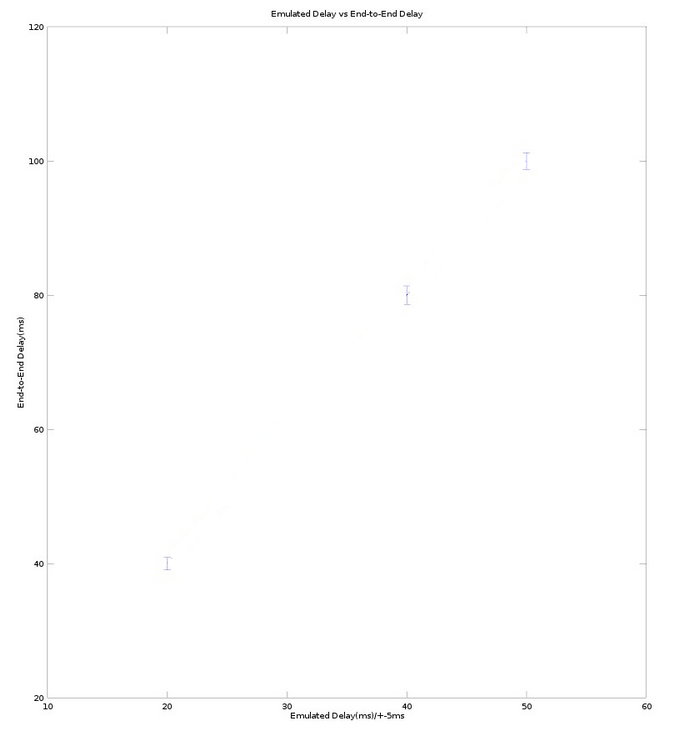
\includegraphics[width=\linewidth]{graph.png}
  \centering
  \caption{Emulation Delays vs End-to-End Delays}
  \label{fig:Topology}
\end{figure}
 
\section{Conclusion}
In this term project, I firstly found the shortest path between $s$ and $d$ by calculating each of the link costs between connected two nodes. In order to find these costs, I wrote different python scripts. While writing these scripts, I firstly learned what a user datagram protocol is. I used socket programming for UDP sockets and learned the concept of multi threading as the nodes were expected to implement multiple tasks at the same time.

In order to find shortest path, I used Dijkstra's Algorithm. According to Dijkstra's algorithm, starting node starts to select the node which has minimum cost among its neighbors and this procedure works cumulatively until reaching the destination node. I found S-R3-D path using this algorithm as the shortest path.

In the experiments, I could not observe a clear and consistent change between emulation delays and end-to-end delays. I was expecting end-to-end delay to increase as I increase the emulation delay. However, they did not increase as I did expected. I believe that the codes that I wrote for measuring the end-to-end delays are okay and so the calculations to find the average values of all the messages sent. Thus, I might have used incorrect tc/netem commands to create emulation delays, which cause us to achieve incorrect end-to-end delays. Unfortunately, I couldn't understand the reason causing that inconsistency between emulation and end-to-end delays yet.

\begin{thebibliography}{00}
\bibitem{b1}A. Kurose and K. W. Ross, Computer networking: a top-down approach. Harlow, Essex: Pearson Education limited, 2013.
\bibitem{b2}A. Malakhov, D. Liu, A. Gorshkov, and T. Wilmarth, “Composable Multi-Threading and Multi-Processing for Numeric Libraries,” Proceedings of the 17th Python in Science Conference, 2018.
\end{thebibliography}

\end{document}